% ─────────────────────────────────────────────────────────────────────────────
\newpage
\section{Graybox Robustness Across Surrogate Models}
\label{sec:ch6_graybox}

% TODO[Kiệt]:
% Goal:
% - Explain graybox robustness as transfer behavior, not just another accuracy table.
% Flow:
% - Start with protocol sanity, then transfer matrices, pairwise comparisons, gap analysis, per-cell analysis, and decomposition.
% Include:
% - Cite active figures/tables from docs/04_figure_table_registry.md, especially currently unreferenced graybox tables/figures if kept.
% Avoid:
% - Overclaiming deployment transfer beyond the surrogate/target protocol.
% Target length: 6-9 pages depending on consolidation.
% ─────────────────────────────────────────────────────────────────────────────

The whitebox results in Section~\ref{sec:ch6_whitebox} show that
AttackDRO++ improves average and held-out robustness over Multi-AT on
\(n=20\) paired seeds. We next test whether this gain also holds under
cross-model transfer, using the graybox protocol of
Section~\ref{sec:ch5_graybox_protocol}. In this setting, adversarial examples
are generated on one checkpoint and evaluated on an independently trained
target checkpoint.

\paragraph{Random-seed checkpoint panel and whitebox sanity check.}

% TODO[Kiệt]:
% Goal:
% - Justify the random-seed checkpoint panel and show it is consistent with the main whitebox trends.
% Flow:
% - Explain the fixed random-seed panel, then interpret `tab:ch6_graybox_whitebox_sanity`.
% Include:
% - State clearly that this is a sanity check, not the main 20-seed whitebox result.
% Avoid:
% - Repeating full Chapter 6.1 results.
% Target length: 2-3 paragraphs.

The graybox analysis uses 20 random-seed checkpoints to define the
surrogate--target evaluation panel. These checkpoints come from four method
families evaluated across five random seeds each and are fixed before graybox
transfer is analyzed. The diagonal sanity check below compares this
random-seed checkpoint panel against the full whitebox panel to verify that the
main method ordering is preserved.

The diagonal entries of the graybox table correspond to the case where
the surrogate and target are the same checkpoint. We use these entries as
a whitebox sanity check. They need not match the main whitebox evaluation
exactly, because the graybox cache uses a balanced
125-image-per-class-per-attack split instead of the full test set for
each attack. However, they should preserve the same method ordering and
remain close in absolute value.

\begin{table}[H]
\centering
\caption{Whitebox sanity check from the graybox pipeline. The \(n=5\)
columns use diagonal graybox entries, where surrogate and target are the
same checkpoint. The \(n=20\) columns report the main whitebox results
from Table~\ref{tab:ch6_aggregate_results}.}
\label{tab:ch6_graybox_whitebox_sanity}
\small
\setlength{\tabcolsep}{6pt}
\renewcommand{\arraystretch}{1.08}
\begin{tabular}{lrrrr}
\toprule
Target method
& Mean(8) \(n=5\)
& Worst(8) \(n=5\)
& Mean(8) \(n=20\)
& Worst(8) \(n=20\) \\
\midrule
PGD-AT
& $61.524$ & $\mathbf{50.384}$ & $60.499$ & $\mathbf{49.656}$ \\
DDN-AT
& $56.922$ & $25.568$ & $56.226$ & $25.957$ \\
Multi-AT
& $62.458$ & $45.584$ & $62.045$ & $45.082$ \\
AttackDRO++ (Ours)
& $\mathbf{62.642}$ & $45.088$ & $\mathbf{62.324}$ & $45.079$ \\
\bottomrule
\end{tabular}
\end{table}

The Mean(8) ordering is identical on both panels --- AttackDRO++ $>$
Multi-AT $>$ PGD-AT $>$ DDN-AT --- and absolute values agree to within
$1.0$~pp. More importantly, the paired Mean(8) delta of AttackDRO++ minus
Multi-AT is $+0.184$~pp on the $n=5$ graybox panel and
$+0.279$~pp on the full $n=20$ panel: both are positive and of the same
order of magnitude. The graybox cache is therefore consistent with the
main evaluation protocol and supports the cross-method analyses below.

\subsection{Cross-Method Transfer Structure}
\label{subsec:ch6_graybox_transfer_structure}

% TODO[Kiệt]:
% Goal:
% - Explain how to read the graybox transfer matrices and what off-diagonal transfer means.
% Flow:
% - Define row/column roles, then interpret aggregate and per-attack matrices.
% Include:
% - Reference `fig:ch6_graybox_transfer_matrix`, `fig:ch6_graybox_transfer_linf`, and `fig:ch6_graybox_transfer_l2`.
% Avoid:
% - Treating diagonal whitebox cells as graybox evidence.
% Target length: 3-5 paragraphs.

We aggregate the per-attack per-class transfer table into a method-level
$4 \times 4$ transfer matrix. Rows index the target method being evaluated, and columns index the
surrogate method that generates adversarial examples. Each cell reports
the target robust accuracy averaged over all matching target--surrogate
seed pairs and the eight evaluation attacks. Higher values indicate that
the row target is more robust to adversarial examples crafted on the
column surrogate.

\begin{figure}[H]
\centering
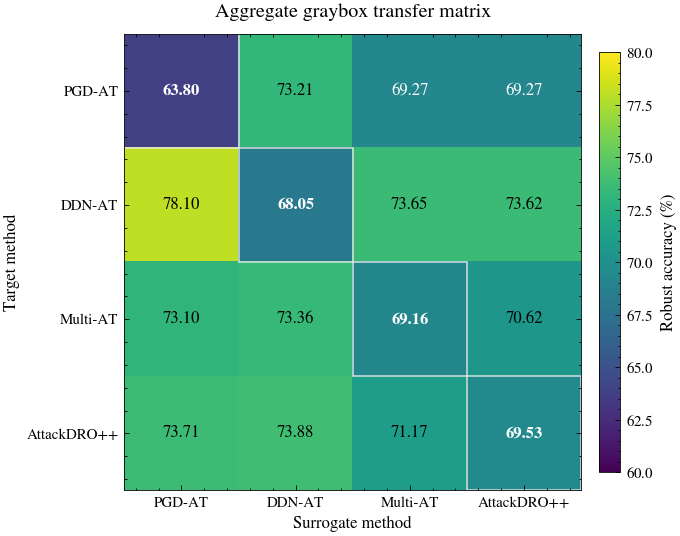
\includegraphics[width=0.78\linewidth]{figures/graybox/graybox_transfer_matrix_4method_aggregate_science_clean.png}
\caption{Method-level graybox transfer matrix on the \(n=5\) panel.
Rows are target methods and columns are surrogate methods. Cell values
are robust accuracy (\%) averaged over seeds and the eight evaluation
attacks.}
\label{fig:ch6_graybox_transfer_matrix}
\end{figure}

Two structural patterns are visible. First, rows ranked by mean
off-diagonal accuracy give DDN-AT ($75.12\%$) $>$ AttackDRO++ ($72.92\%$)
$>$ Uniform Multi-AT ($72.36\%$) $>$ PGD-AT ($70.59\%$). The DDN-AT
row is highest not because DDN-AT is the strongest defense --- its
whitebox Mean(8) is the lowest of the four --- but because $\ell_\infty$
adversarial examples generated by other surrogates transfer poorly to a
DDN-AT target whose decision boundary is shaped by $\ell_2$ training.
Section~\ref{subsec:ch6_paired_graybox_comparisons} quantifies this structural inflation
explicitly through the whitebox--graybox gap. Second, the AttackDRO++
row is consistently above the Uniform Multi-AT row for every surrogate,
with cross-method gaps ranging from $+0.17$~pp (DDN-AT surrogate) to
$+0.61$~pp (PGD-AT surrogate). The whitebox advantage of AttackDRO++
over Uniform Multi-AT therefore persists when adversarial examples are
crafted on independently trained surrogates.

The aggregate transfer matrix hides important attack-family structure.
Figures~\ref{fig:ch6_graybox_transfer_linf} and~\ref{fig:ch6_graybox_transfer_l2}
therefore disaggregate the transfer behavior into the four
\(\ell_\infty\)-oriented attacks and the four \(\ell_2\)-oriented attacks.
This grouping makes the specialist behavior more explicit. 

\begin{figure}[H]
\centering
\begin{minipage}{0.48\linewidth}
  \centering
  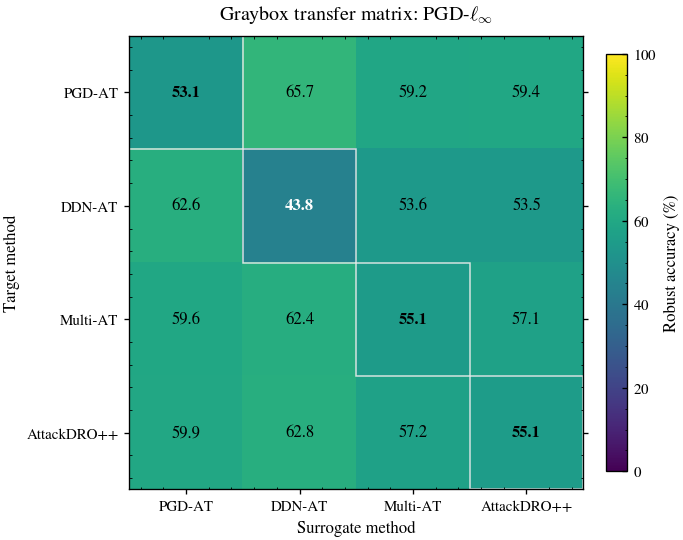
\includegraphics[width=\linewidth]{figures/graybox/transfer_matrix_4method_pgd20_ce_science_clean.png}
  \\ \footnotesize (a) PGD-\(\ell_\infty\)
\end{minipage}\hfill
\begin{minipage}{0.48\linewidth}
  \centering
  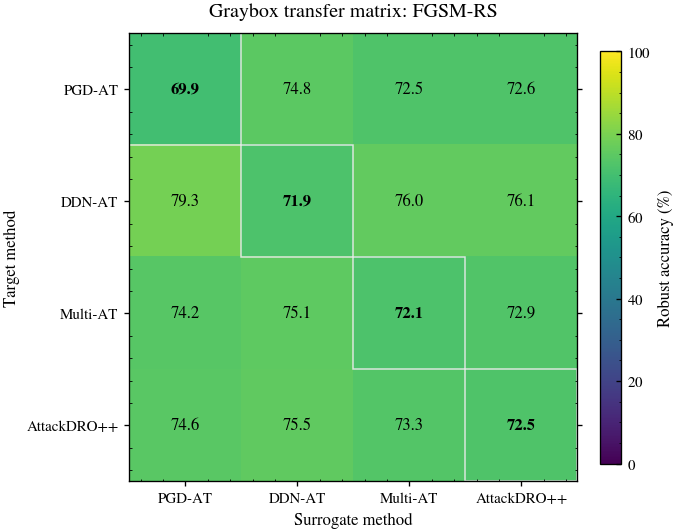
\includegraphics[width=\linewidth]{figures/graybox/transfer_matrix_4method_fgsm_rs_science_clean.png}
  \\ \footnotesize (b) FGSM-RS
\end{minipage}

\vspace{0.6em}

\begin{minipage}{0.48\linewidth}
  \centering
  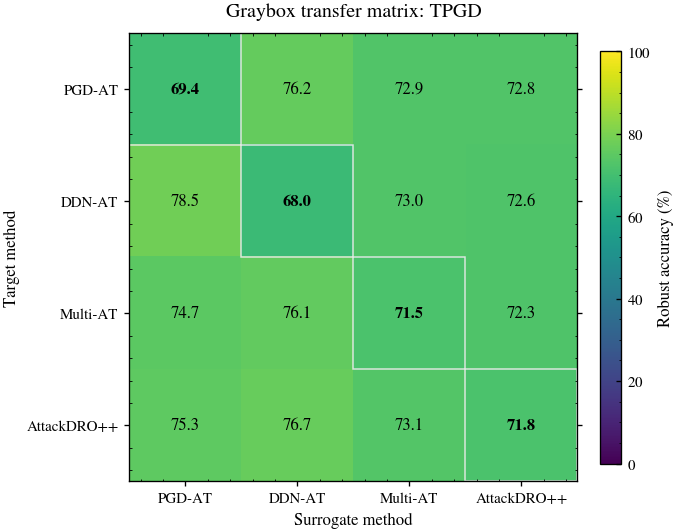
\includegraphics[width=\linewidth]{figures/graybox/transfer_matrix_4method_tpgd_science_clean.png}
  \\ \footnotesize (c) TPGD
\end{minipage}\hfill
\begin{minipage}{0.48\linewidth}
  \centering
  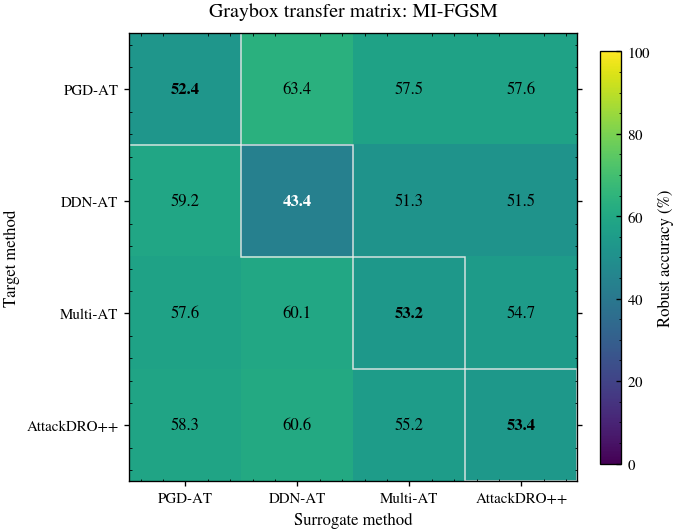
\includegraphics[width=\linewidth]{figures/graybox/transfer_matrix_4method_mifgsm_science_clean.png}
  \\ \footnotesize (d) MI-FGSM
\end{minipage}

\caption{Per-attack graybox transfer matrices for the
\(\ell_\infty\)-oriented attacks. Rows are target methods and columns
are surrogate methods; cells report robust accuracy (\%).}
\label{fig:ch6_graybox_transfer_linf}
\end{figure}

On the
\(\ell_\infty\) attacks, this advantage disappears: PGD-AT and
AttackDRO++ are more competitive, and AttackDRO++ remains closer to the
balanced Multi-AT profile. Thus, the per-attack matrices show that
DDN-AT's strong graybox row average should be interpreted as
family-specific transfer specialization rather than uniform robustness.

\begin{figure}[H]
\centering
\begin{minipage}{0.48\linewidth}
  \centering
  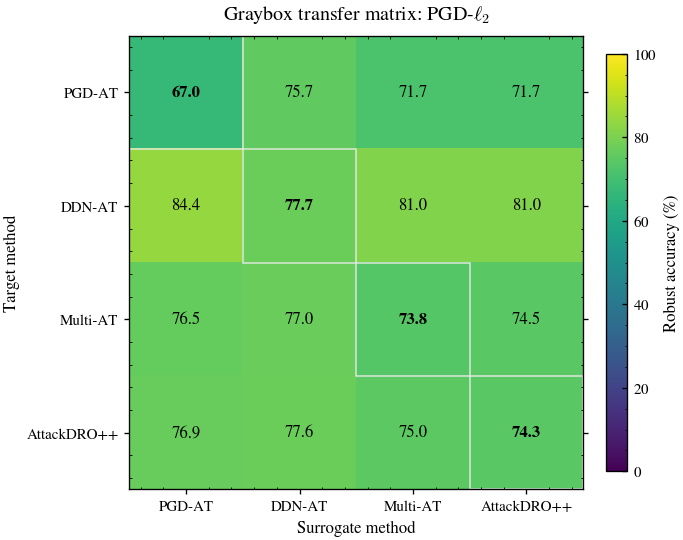
\includegraphics[width=\linewidth]{figures/graybox/transfer_matrix_4method_pgd_l2_science_clean.png}
  \\ \footnotesize (a) PGD-\(\ell_2\)
\end{minipage}\hfill
\begin{minipage}{0.48\linewidth}
  \centering
  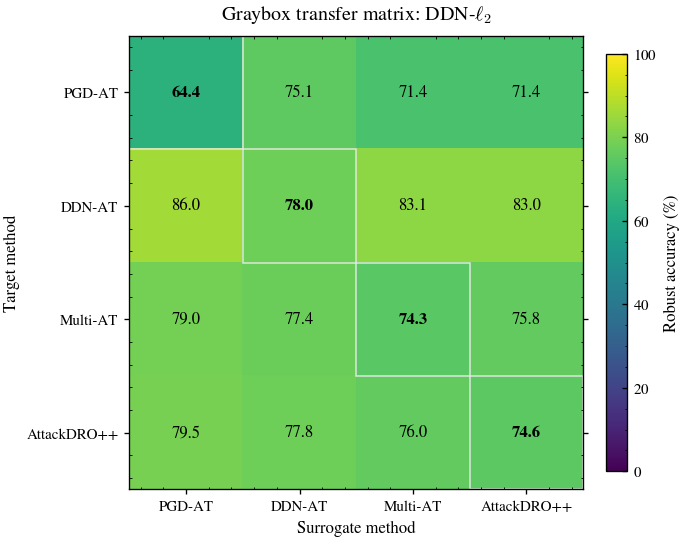
\includegraphics[width=\linewidth]{figures/graybox/transfer_matrix_4method_ddn_l2_science_clean.png}
  \\ \footnotesize (b) DDN-\(\ell_2\)
\end{minipage}

\vspace{0.6em}

\begin{minipage}{0.48\linewidth}
  \centering
  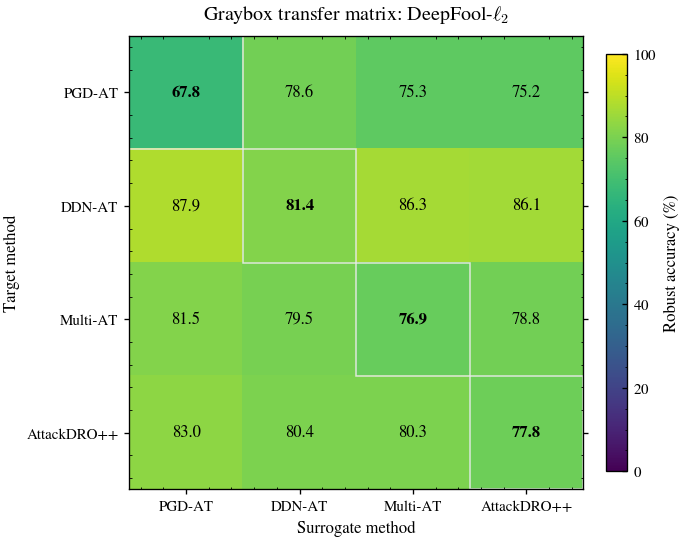
\includegraphics[width=\linewidth]{figures/graybox/transfer_matrix_4method_deepfool_l2_science_clean.png}
  \\ \footnotesize (c) DeepFool-\(\ell_2\)
\end{minipage}\hfill
\begin{minipage}{0.48\linewidth}
  \centering
  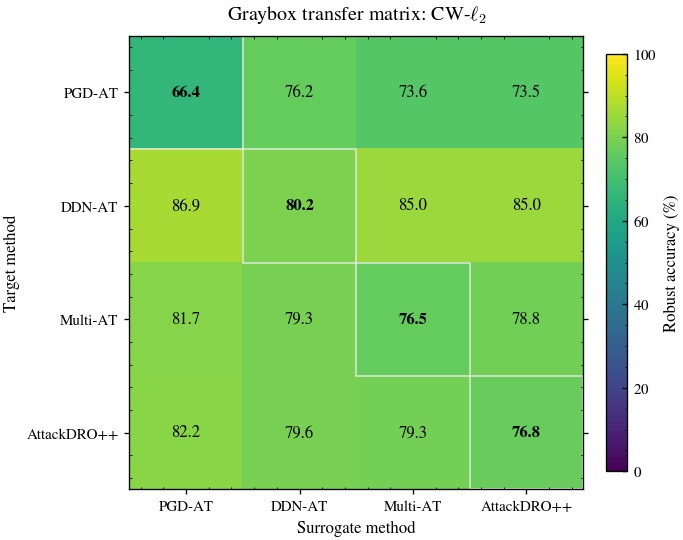
\includegraphics[width=\linewidth]{figures/graybox/transfer_matrix_4method_cw_l2_science_clean.png}
  \\ \footnotesize (d) CW-\(\ell_2\)
\end{minipage}

\caption{Per-attack graybox transfer matrices for the
\(\ell_2\)-oriented attacks. Rows are target methods and columns are
surrogate methods; cells report robust accuracy (\%).}
\label{fig:ch6_graybox_transfer_l2}
\end{figure}
On the \(\ell_2\) attacks, the DDN-AT target row is consistently strong,
especially when attacks are transferred from PGD-AT, Multi-AT, or
AttackDRO++ surrogates. This indicates that DDN-AT's high aggregate
graybox score is driven mainly by \(\ell_2\)-family transfer behavior,
rather than by uniformly strong robustness across both attack geometries.
AttackDRO++ remains closer to the balanced Multi-AT profile, while still
improving over Multi-AT on most \(\ell_2\)-oriented transfer cells.


\subsection{Paired Graybox Comparisons: Does the Whitebox Advantage Carry Over?}
\label{subsec:ch6_paired_graybox_comparisons}

% TODO[Kiệt]:
% Goal:
% - Compare AttackDRO++ against the strongest uniform multi-attack baseline under graybox transfer.
% Flow:
% - Interpret paired graybox tests, then identify where the advantage is robust or limited.
% Include:
% - Reference `tab:ch6_paired_graybox_two_panel` and `tab:ch6_graybox_attack_family`.
% Avoid:
% - Ignoring corrected p-values or effect size when discussing differences.
% Target length: 3-5 paragraphs.

The main graybox comparison is between AttackDRO++ and Multi-AT.
Both methods train on the same source attacks
$\{\text{PGD-}\ell_\infty,\ \text{DDN-}\ell_2\}$ and use the same backbone
and schedule; they differ only in the use of latent clustering, gradient
fingerprints, and the anchored Cluster-DRO objective.

We use the symmetric paired test that has already been described in
Section~\ref{sec:ch5_graybox_protocol}: for every triple
$(\text{target seed},\ \text{surrogate seed},\ \text{attack})$, we pair
the configuration ``AttackDRO++ as target, Multi-AT as surrogate'' against
its mirror ``Multi-AT as target, AttackDRO++ as surrogate'' and compute
the per-triple difference. As the results, $n = 5 \times 5 \times 8 = 200$
paired pairs make the comparison invariant to which method is chosen as
the surrogate.
\begin{table}[H]
\centering
\caption{Paired graybox comparisons. Each row uses $n=200$ paired
target--surrogate--attack triples. Positive $\Delta$ favors the reference
method named in the panel heading.}
\label{tab:ch6_paired_graybox_two_panel}
\begin{tabular}{lcccccc}
\toprule
Compared method
& \multicolumn{2}{c}{Accuracy}
& $\Delta$
& $d_z$
& $t$
& $p$ \\
\cmidrule(lr){2-3}
& Reference
& Baseline
& (pp)
& 
& 
&  \\
\midrule

\multicolumn{7}{l}{\textit{AttackDRO++ (Ours) vs. baselines}} \\
\midrule
Multi-AT
& 71.17
& 70.62
& +0.549
& 0.42
& 5.96
& \textbf{$1.1{\times}10^{-8}$} \\

PGD-AT
& 73.71
& 69.27
& \textbf{+4.435}
& 1.33
& 18.78
& \textbf{$6.1{\times}10^{-46}$} \\

DDN-AT
& 73.88
& 73.62
& +0.258
& 0.04
& 0.60
& 0.549 \\

\midrule
\multicolumn{7}{l}{\textit{Multi-AT vs. single-attack baselines}} \\
\midrule
PGD-AT
& 73.10
& 69.27
& \textbf{+3.829}
& 1.19
& 16.89
& \textbf{$2.7{\times}10^{-40}$} \\

DDN-AT
& 73.36
& 73.65
& $-0.292$
& $-0.05$
& $-0.67$
& 0.504 \\

\bottomrule
\end{tabular}
\end{table}

The AttackDRO++ vs. Multi-AT contrast is the headline result of
this section: under symmetric cross-method graybox transfer,
AttackDRO++ improves onMulti-AT by $+0.549$~pp at
$p \approx 1.1 \times 10^{-8}$, with a small-to-medium paired effect size
of $d_z \approx 0.42$. This effect is roughly twice the corresponding
whitebox delta of $+0.279$~pp on the same seed panel and is significant
at far stricter levels. The Cluster-DRO improvement therefore
\emph{strengthens} rather than disappears under graybox transfer,
indicating that the gain originates from a broader cross-attack
robustness profile rather than from a defense narrowly tuned to
AttackDRO++'s own gradients.

The single-attack contrasts confirm the expected specialist--versus--balanced
pattern. AttackDRO++ improves on PGD-AT by $+4.44$~pp at
$p < 10^{-45}$ ($d_z = 1.33$, a large effect), tracking the whitebox
trend that PGD-AT loses heavily on the $\ell_2$ family it does not train
against. The AttackDRO++ vs.\ DDN-AT contrast is statistically
indistinguishable from zero ($+0.26$~pp, $p = 0.55$); this reflects the
DDN-AT graybox inflation discussed above, not actual parity. We dissect
this asymmetry in Section~\ref{subsec:ch6_paired_graybox_comparisons}.

\paragraph{Per-attack transfer behavior.}

% TODO[Kiệt]:
% Goal:
% - Identify which attacks drive graybox transfer differences.
% Flow:
% - Discuss per-attack table, then connect attack-family behavior to whitebox findings.
% Include:
% - Reference `tab:ch6_graybox_per_attack` if retained in the main flow.
% Avoid:
% - Duplicating the transfer-matrix discussion.
% Target length: 2-4 paragraphs.

To check whether the $+0.549$~pp Mean(8) gain over Multi-AT is
broad or concentrated, we report paired graybox deltas attack by attack
on the same $n=200$ pair set. Each attack contributes $25$ paired
triples (one per surrogate--target seed combination).

\begin{table}[H]
\centering
\caption{Per-attack symmetric graybox comparison between AttackDRO++
and Multi-AT. Each attack uses \(n=25\) paired seed combinations.
Bold deltas are significant at \(p<0.05\).}
\label{tab:ch6_graybox_per_attack}
\small
\setlength{\tabcolsep}{4pt}
\renewcommand{\arraystretch}{1.10}
\begin{tabular}{llrrrr}
\toprule
Attack          & Family              & A mean (\%) & B mean (\%) & $\Delta$ (pp) & $p$ \\
\midrule
FGSM-RS         & held-out $\ell_\infty$ & $73.32$ & $72.86$ & $\mathbf{+0.454}$ & $0.0114$ \\
PGD-$\ell_\infty$ & seen $\ell_\infty$    & $57.17$ & $57.07$ & $+0.102$ & $0.307$  \\
TPGD            & held-out $\ell_\infty$ & $73.09$ & $72.30$ & $\mathbf{+0.790}$ & $0.0240$ \\
MI-FGSM         & held-out $\ell_\infty$ & $55.20$ & $54.75$ & $\mathbf{+0.458}$ & $0.0022$ \\
\midrule
PGD-$\ell_2$    & held-out $\ell_2$      & $74.97$ & $74.53$ & $\mathbf{+0.432}$ & $0.0373$ \\
DDN-$\ell_2$    & seen $\ell_2$          & $76.04$ & $75.79$ & $+0.256$ & $0.341$  \\
DeepFool-$\ell_2$ & held-out $\ell_2$    & $80.29$ & $78.82$ & $\mathbf{+1.469}$ & $0.0002$ \\
CW-$\ell_2$     & held-out $\ell_2$      & $79.26$ & $78.83$ & $+0.429$ & $0.249$  \\
\bottomrule
\end{tabular}
\end{table}

AttackDRO++ produces a positive paired delta on all eight attacks. Five
of these deltas are individually significant at $p < 0.05$, and the gain
is largest on DeepFool-$\ell_2$ ($+1.47$~pp, $p = 1.6\times 10^{-4}$),
the most local-gradient $\ell_2$ attack and the held-out attack on which
the whitebox gain over Multi-AT was also largest. The two seen
attacks (PGD-$\ell_\infty$ and DDN-$\ell_2$) contribute small,
non-significant gains, consistent with the fact that both methods
already train against these attacks. The graybox Mean(8) gain is
therefore distributed across attack families rather than concentrated on
one family.

We aggregate the per-attack deltas into the four attack groups defined
in Section~\ref{sec:ch5_evaluation_metrics} to compare the cross-method graybox
profile across all four methods.

\begin{table}[H]
\centering
\caption{Cross-method graybox accuracy by attack family. Values are
off-diagonal target accuracy (\%) averaged over the \(n=5\) panel.
Bold values mark the best method in each column.}
\label{tab:ch6_graybox_attack_family}
\small
\setlength{\tabcolsep}{6pt}
\renewcommand{\arraystretch}{1.08}
\begin{tabular}{lrrrrr}
\toprule
Target method     & Seen $\ell_\infty$ & Seen $\ell_2$ & Heldout $\ell_\infty$ & Heldout $\ell_2$ & Mean(8) \\
\midrule
PGD-AT & $\mathbf{61.48}$ & $72.61$ & $68.93$           & $74.60$           & $70.59$ \\
DDN-AT      & $56.58$          & $\mathbf{84.03}$ & $68.60$ & $\mathbf{84.85}$  & $\mathbf{75.12}$ \\
Multi-AT  & $59.71$          & $77.40$          & $68.64$ & $78.62$           & $72.36$ \\
AttackDRO++ (Ours) & $59.96$          & $77.78$          & $\mathbf{69.18}$ & $79.35$ & $72.92$ \\
\bottomrule
\end{tabular}
\end{table}

The family decomposition makes three points concrete. The held-out
$\ell_\infty$ column has AttackDRO++ at the top ($69.18\%$) by a small
but consistent margin over the other three methods. The held-out
$\ell_2$ column is dominated by DDN-AT ($84.85\%$), with AttackDRO++
($79.35\%$) ranked second and improving on Multi-AT by
$+0.73$~pp. The seen $\ell_2$ column shows the same pattern. The seen
$\ell_\infty$ column favors PGD-AT, again by structure: surrogates
generate strong PGD-$\ell_\infty$ adversarial examples, and only PGD-AT
is robust to them. AttackDRO++ is the only method that is at or above
Multi-AT on every attack family, while DDN-AT and PGD-AT each
remain narrow specialists under transfer.

\paragraph{Whitebox--graybox gap and specialist inflation.}

% TODO[Kiệt]:
% Goal:
% - Explain the gap between direct whitebox robustness and transferred robustness.
% Flow:
% - Define the gap sign, interpret `tab:ch6_graybox_gap`, then use heatmaps for method-specific patterns.
% Include:
% - Reference gap heatmaps from `fig:ch6_graybox_gap_ddnat` to `fig:ch6_graybox_gap_attackdropp`.
% - Add caption polish later for sign/unit/averaging conditions.
% Avoid:
% - Treating large whitebox scores alone as evidence of transferable robustness.
% Target length: 3-5 paragraphs.

The DDN-AT target row in Figure~\ref{fig:ch6_graybox_transfer_matrix} and
the DDN-AT row in Table~\ref{tab:ch6_graybox_attack_family} are the highest
under graybox transfer,
even though DDN-AT has the lowest whitebox Mean(8) on both the $n=5$ and
the full $n=20$ panels. We resolve this apparent contradiction by
quantifying the gap between whitebox and cross-method graybox accuracy
for each method. A large positive gap indicates that a defense looks
much stronger under graybox transfer than under direct whitebox attack,
which is a signature of a structural transfer mismatch rather than a
broader robustness profile.

\begin{table}[H]
\centering
\caption{Whitebox--graybox gap by target method on the \(n=5\) panel.
The gap is cross-method graybox Mean(8) minus diagonal whitebox Mean(8).}
\label{tab:ch6_graybox_gap}
\small
\setlength{\tabcolsep}{8pt}
\renewcommand{\arraystretch}{1.08}
\begin{tabular}{lrrr}
\toprule
Target method     & Whitebox Mean(8) & Graybox Mean(8) & Gap (pp) \\
\midrule
PGD-AT & $61.52$ & $70.59$ & $\phantom{0}+9.06$  \\
DDN-AT      & $56.92$ & $75.12$ & $\mathbf{+18.20}$   \\
Multi-AT  & $62.46$ & $72.36$ & $\phantom{0}+9.90$  \\
AttackDRO++ (Ours) & $\mathbf{62.64}$ & $72.92$ & $+10.27$   \\
\bottomrule
\end{tabular}
\end{table}

PGD-AT, Multi-AT, and AttackDRO++ all show a comparable
whitebox--graybox gap of approximately $9$--$10$~pp, indicating that
adversarial examples crafted on alternate surrogates are weaker than
those crafted directly on the target by a roughly constant amount.
DDN-AT, by contrast, gains $+18.20$~pp under graybox transfer, almost
twice the gap of any other method. Its row-leading graybox accuracy is therefore not evidence of a stronger defense; it is an artifact of
how poorly $\ell_\infty$ adversarial examples generated by PGD-AT, Multi-AT, and AttackDRO++ surrogates transfer to a
purely-$\ell_2$-trained target. AttackDRO++ retains the highest whitebox
Mean(8) of the four methods while exhibiting a graybox gap that is only
$+0.37$~pp larger than that of Multi-AT --- consistent with a
balanced cross-attack defense rather than a transfer-favored
specialist.

The per-(class \(\times\) attack) whitebox--graybox gap heatmaps in
Figures~\ref{fig:ch6_graybox_gap_ddnat}--\ref{fig:ch6_graybox_gap_attackdropp}
make the specialist-inflation effect concrete. Cell values are computed
as graybox accuracy minus whitebox accuracy, so positive values indicate
that transferred attacks are weaker than direct whitebox attacks on the
same target.

\begin{figure}[H]
\centering
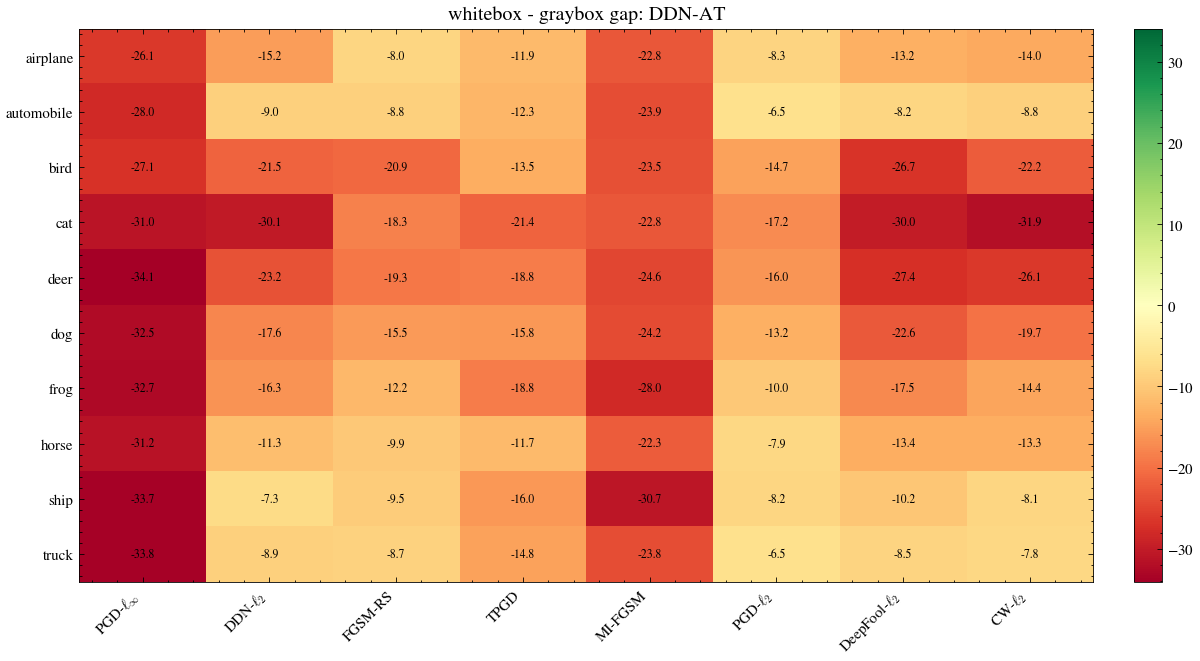
\includegraphics[width=\linewidth]{figures/graybox/whitebox_graybox_gap_DDNAT.png}
\caption{Whitebox--graybox gap heatmap for DDN-AT.}
\label{fig:ch6_graybox_gap_ddnat}
\end{figure}

\begin{figure}[H]
\centering
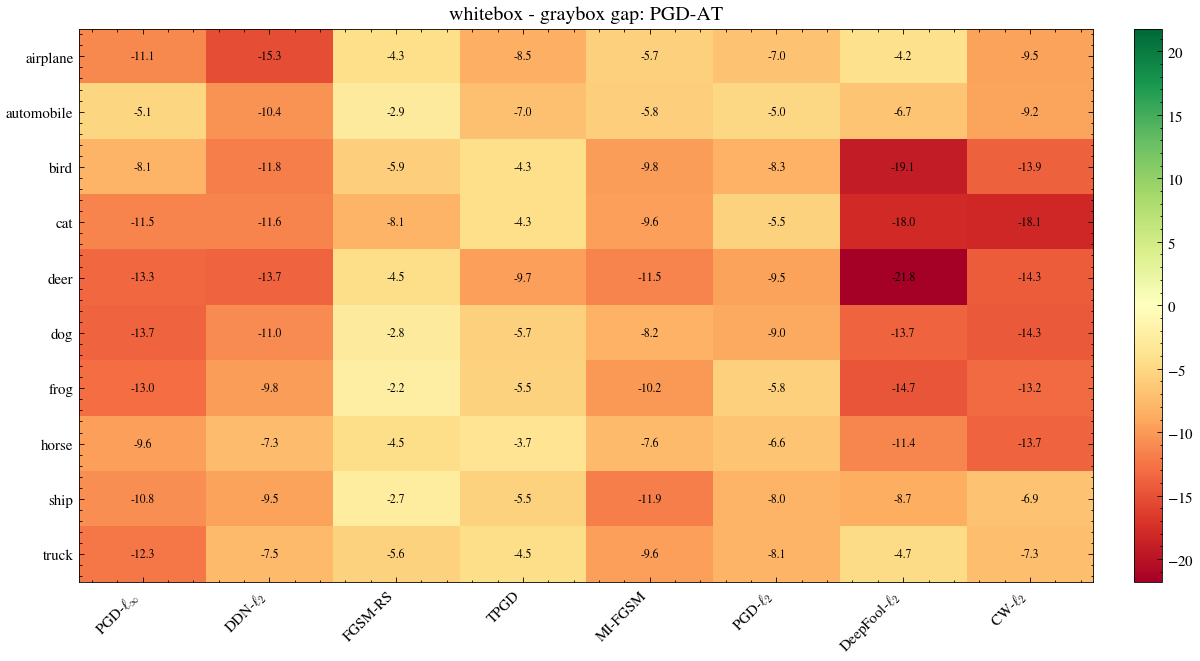
\includegraphics[width=\linewidth]{figures/graybox/whitebox_graybox_gap_PGDAT.png}
\caption{Whitebox--graybox gap heatmap for PGD-AT.}
\label{fig:ch6_graybox_gap_pgdat}
\end{figure}

\begin{figure}[H]
\centering
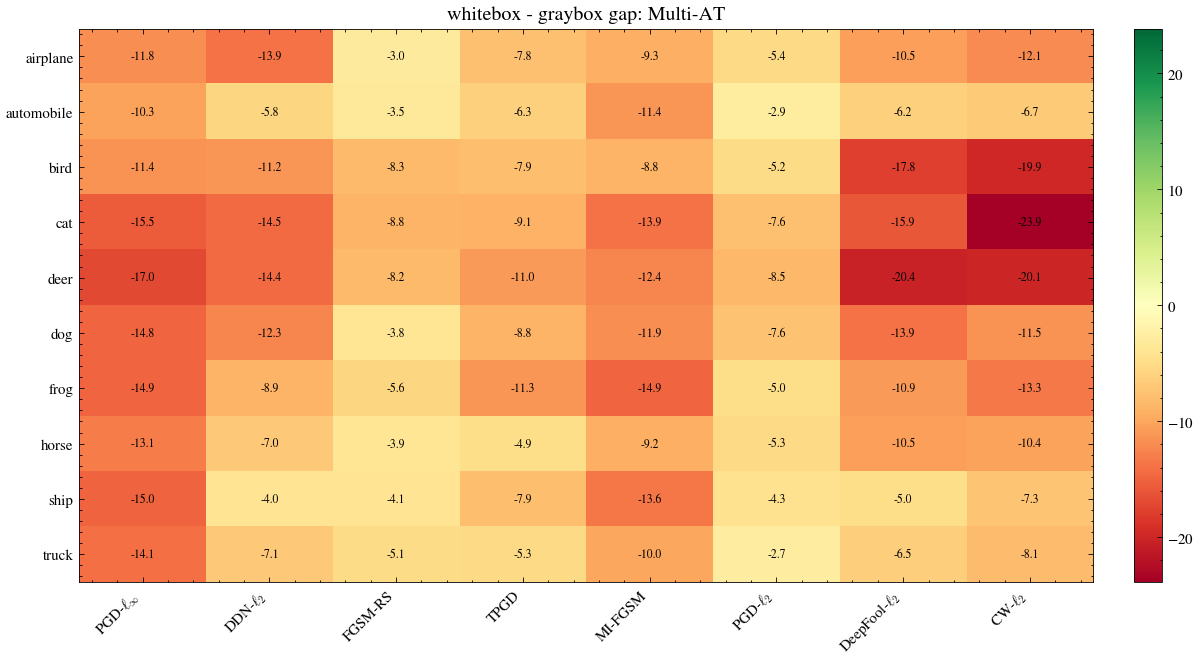
\includegraphics[width=\linewidth]{figures/graybox/whitebox_graybox_gap_MultiAT.png}
\caption{Whitebox--graybox gap heatmap for Multi-AT.}
\label{fig:ch6_graybox_gap_multiat}
\end{figure}

\begin{figure}[H]
\centering
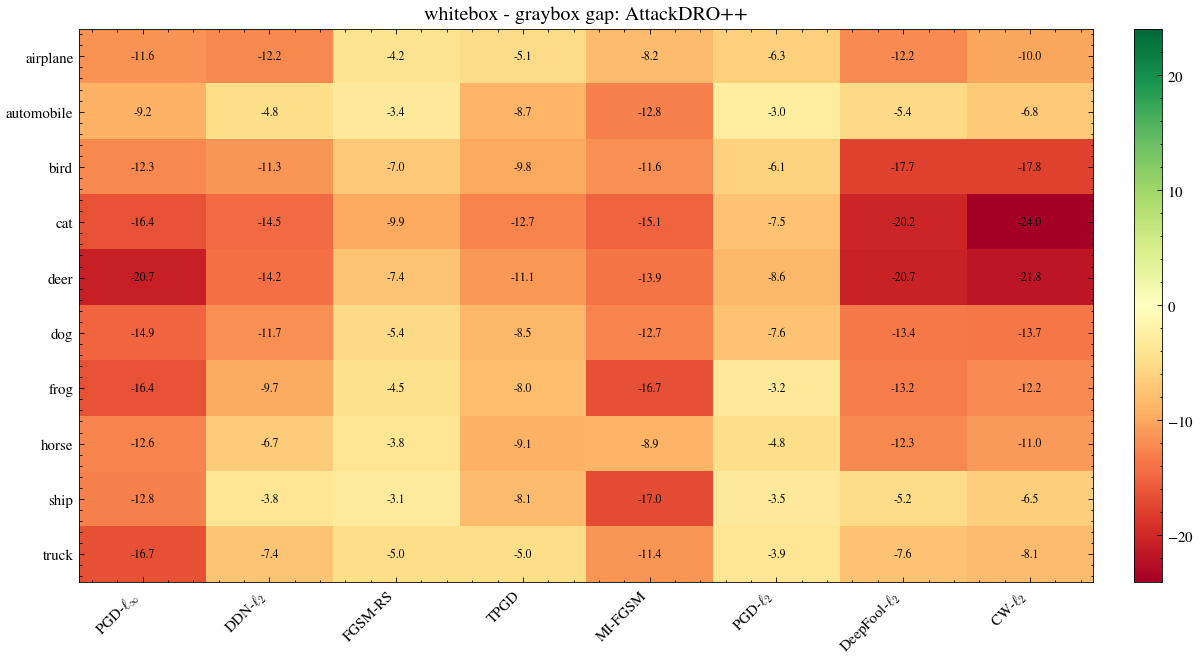
\includegraphics[width=\linewidth]{figures/graybox/whitebox_graybox_gap_AttackDROpp.png}
\caption{Whitebox--graybox gap heatmap for AttackDRO++ (Ours).}
\label{fig:ch6_graybox_gap_attackdropp}
\end{figure}

DDN-AT exhibits broad positive gaps on the \(\ell_\infty\)-oriented
attack columns, indicating that its high graybox score is partly driven
by weak transfer from \(\ell_\infty\) surrogates rather than uniformly
strong robustness. PGD-AT, Multi-AT, and AttackDRO++ show smaller and
more balanced gap patterns, with AttackDRO++ avoiding the severe
specialist inflation observed for DDN-AT.
\subsection{Class-Level Transfer Patterns}
\label{subsec:ch6_class_level_transfer_patterns}

% TODO[Kiệt]:
% Goal:
% - Explain fine-grained graybox gains and failures by class and attack.
% Flow:
% - Interpret `tab:ch6_graybox_per_cell`, then use delta heatmaps to show where gains concentrate.
% Include:
% - Reference `fig:ch6_graybox_delta_multiat`, `fig:ch6_graybox_delta_pgdat`, and `fig:ch6_graybox_delta_ddnat` if all remain in the main flow.
% Avoid:
% - Listing every class-attack cell.
% Target length: 3-5 paragraphs.

We complement the aggregate analysis with a paired per-cell test. For
each of the $80$ attack--class cells, we compare the graybox accuracy of
the AttackDRO++ target against each baseline target across the five
training seeds (each cell pairs $n = 5$ seeds). A two-sided paired
$t$-test is computed per cell.

\begin{table}[H]
\centering
\caption{Per-(class \(\times\) attack) graybox tests comparing
AttackDRO++ against each baseline. \(\Delta\) is computed as
AttackDRO++ minus the baseline.}
\label{tab:ch6_graybox_per_cell}
\footnotesize
\setlength{\tabcolsep}{4.5pt}
\renewcommand{\arraystretch}{1.18}
\begin{tabular}{lccccc}
\toprule
Baseline
& Positive cells
& Sign-test
& Mean
& Significant cells
& Bottom-10 \\
& \((\Delta>0)\)
& \(p\)
& \(\Delta\) (pp)
& AttackDRO++ / Baseline
& lift (pp) \\
\midrule
Multi-AT
& $59/80$
& $\mathbf{1.3{\times}10^{-5}}$
& $+0.557$
& $\phantom{0}2 \,/\, \phantom{0}3$
& $+0.779$ \\

PGD-AT
& $52/80$
& $\mathbf{4.8{\times}10^{-3}}$
& $+2.332$
& $34 \,/\, 12$
& $+1.329$ \\

DDN-AT
& $27/80$
& $\mathbf{2.4{\times}10^{-3}}$
& $-2.206$
& $16 \,/\, 32$
& $+0.709$ \\
\bottomrule
\end{tabular}
\end{table}

Three observations follow. First, AttackDRO++ exceeds Multi-AT on
$59$ of $80$ cells with a mean per-cell delta of $+0.557$~pp, in close
agreement with the $+0.549$~pp aggregate from
Table~\ref{tab:ch6_paired_graybox_two_panel}. Cell-level significance is sparse
($2$ vs.\ $3$ cells reach $p < 0.05$ in either direction), as expected
under the $n = 5$ per-cell sample size and the small absolute deltas;
the bulk of the evidence for AttackDRO++ is therefore the
\emph{distributional} shift across many cells rather than a few cell-level
landslides.

Second, the bottom-10 lift is positive in all three contrasts. The cells
on which Multi-AT, PGD-AT, and DDN-AT are weakest concentrate on
the cat, deer, dog, and bird classes under MI-FGSM, PGD-$\ell_\infty$,
and PGD-$\ell_2$. AttackDRO++ improves on Multi-AT by
$+0.779$~pp on Multi-AT's worst $10$ cells, and improves on
PGD-AT by $+1.329$~pp on PGD-AT's worst $10$ cells.

Third, the AttackDRO++ vs.\ DDN-AT cell-level comparison ($-2.21$~pp on
average, $32$ cells favoring DDN-AT at $p<0.05$) is the per-cell
counterpart of the DDN-AT graybox inflation: most of DDN-AT's wins are
on $\ell_2$ cells, while AttackDRO++ retains the wins it needs on the
$\ell_\infty$ cells that DDN-AT collapses on under whitebox attack
(Section~\ref{subsec:ch6_per_attack_accuracy}).

The heatmaps in
Figures~\ref{fig:ch6_graybox_delta_multiat}--\ref{fig:ch6_graybox_delta_ddnat} visualize these patterns
explicitly: green cells favor AttackDRO++, red cells favor the baseline.
The AttackDRO++ vs.\ Multi-AT heatmap is broadly green and small
in magnitude; the AttackDRO++ vs.\ PGD-AT heatmap is broadly green with
a few large red cells on $\ell_\infty$ attacks where PGD-AT specializes;
and the AttackDRO++ vs.\ DDN-AT heatmap is mixed.

\begin{figure}[H]
\centering
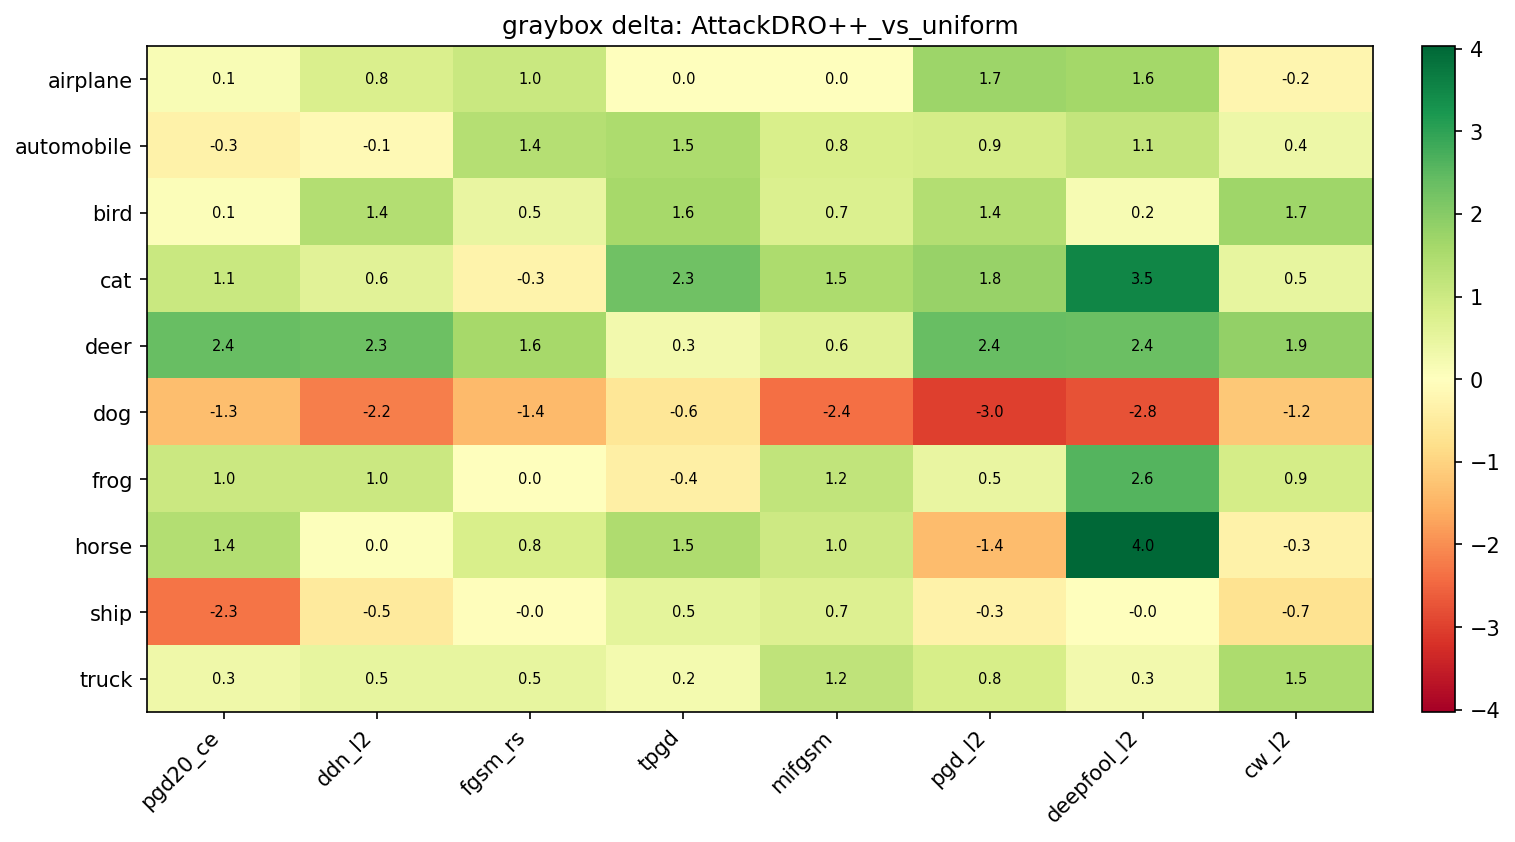
\includegraphics[width=\linewidth]{figures/graybox/graybox_delta_per_class_attack_AttackDRO++_vs_uniform.png}
\caption{Per-(class \(\times\) attack) graybox delta heatmap for
AttackDRO++ (Ours) minus Multi-AT. Green favors AttackDRO++ (Ours); red favors
Multi-AT.}
\label{fig:ch6_graybox_delta_multiat}
\end{figure}

\begin{figure}[H]
\centering
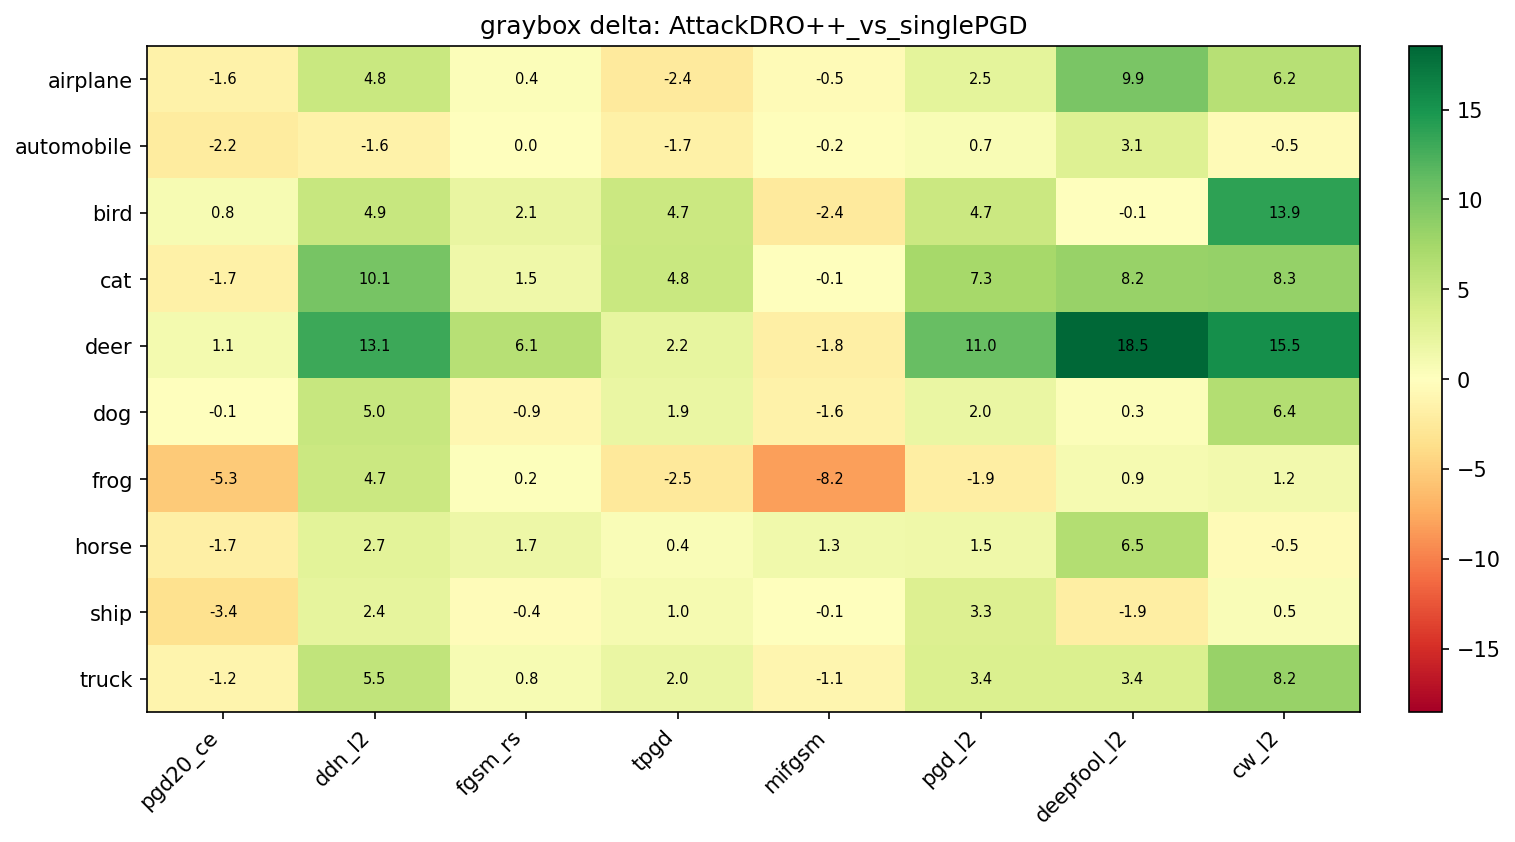
\includegraphics[width=\linewidth]{figures/graybox/graybox_delta_per_class_attack_AttackDRO++_vs_singlePGD.png}
\caption{Per-(class \(\times\) attack) graybox delta heatmap for
AttackDRO++ (Ours) minus PGD-AT. Green favors AttackDRO++ (Ours); red favors PGD-AT.}
\label{fig:ch6_graybox_delta_pgdat}
\end{figure}

\begin{figure}[H]
\centering
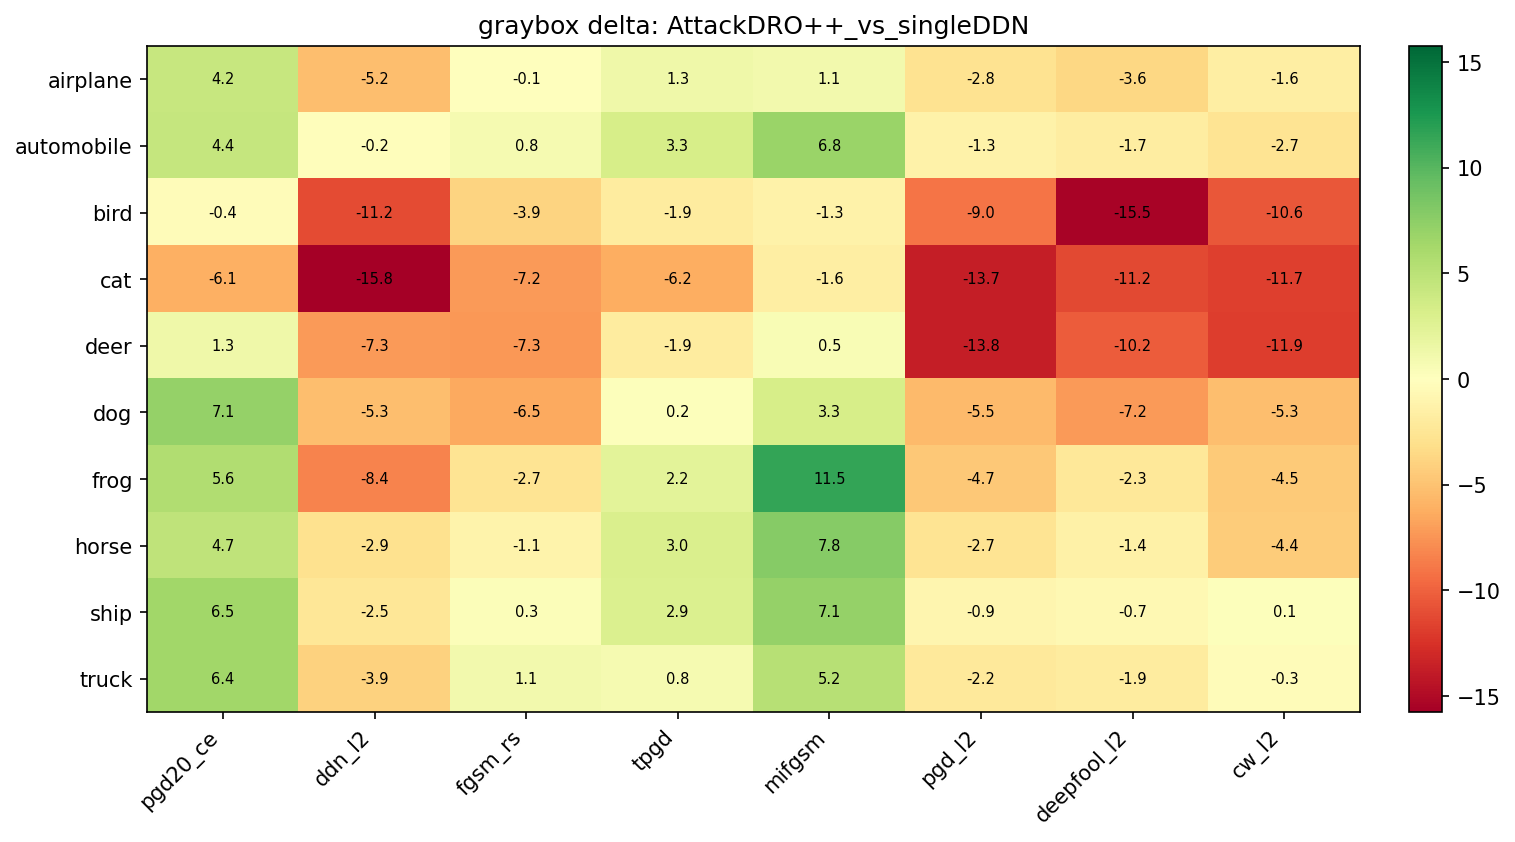
\includegraphics[width=\linewidth]{figures/graybox/graybox_delta_per_class_attack_AttackDRO++_vs_singleDDN.png}
\caption{Per-(class \(\times\) attack) graybox delta heatmap for
AttackDRO++ (Ours) minus DDN-AT. Green favors AttackDRO++ (Ours); red favors DDN-AT.}
\label{fig:ch6_graybox_delta_ddnat}
\end{figure}

\newpage
\paragraph{Method contribution decomposition.}

% TODO[Kiệt]:
% Goal:
% - Explain the contribution split between multi-attack training and Cluster-DRO components.
% Flow:
% - Interpret the decomposition table first, then use the figure as visual support.
% Include:
% - Reference `tab:ch6_graybox_decomposition` and `fig:ch6_method_decomposition` if kept.
% Avoid:
% - Treating decomposition as causal proof beyond the available comparisons.
% Target length: 2-4 paragraphs.

The whitebox results of Section~\ref{sec:ch6_whitebox} compare AttackDRO++
against Multi-AT and against the two single-attack baselines as
three separate contrasts. Under graybox transfer, we can additionally
ask how much of the AttackDRO++ improvement over each single-attack
baseline is contributed by multi-attack training (the Multi-AT
component) versus the Cluster-DRO objective (the AttackDRO++ component
on top of Multi-AT). We decompose the total
AttackDRO++ vs.\ single-attack delta as
\[
\Delta_{\text{total}}
\;=\;
\underbrace{(\text{Multi-AT}) - (\text{single-AT})}_{\Delta_{\text{multi-attack}}}
\;+\;
\underbrace{(\text{AttackDRO++}) - (\text{Multi-AT})}_{\Delta_{\text{Cluster-DRO}}},
\]
and report this decomposition for whitebox Mean(8), cross-method graybox
Mean(8), and the bottom-10-cell cross-method graybox average (the average
graybox accuracy on the ten attack--class cells in which the target is
weakest). The bottom-10 metric is included because it isolates worst-cell
behavior, which is most sensitive to the AttackDRO++ objective.

\begin{table}[H]
\centering
\caption{AttackDRO++ (Ours) gain decomposition. Values are percentage-point changes.}
\label{tab:ch6_graybox_decomposition}
\small
\setlength{\tabcolsep}{6pt}
\renewcommand{\arraystretch}{1.10}
\begin{tabular}{llrrr}
\toprule
Metric & Base & Multi-AT & DRO++ & Total \\
\midrule
Whitebox Mean(8)        & PGD-AT & $+0.934$ & $+0.184$ & $+1.118$ \\
Whitebox Mean(8)        & DDN-AT & $+5.536$ & $+0.184$ & $+5.720$ \\
\midrule
Cross-graybox Mean(8)   & PGD-AT & $+1.775$ & $+0.557$ & $+2.332$ \\
Cross-graybox Mean(8)   & DDN-AT & $-2.763$ & $+0.557$ & $-2.206$ \\
\midrule
Bottom-10 graybox       & PGD-AT & $+0.530$ & $+0.799$ & $+1.329$ \\
Bottom-10 graybox       & DDN-AT & $-0.090$ & $+0.799$ & $+0.709$ \\
\bottomrule
\end{tabular}
\end{table}
The Cluster-DRO effect (column 4) is positive on every metric and
decomposition path, ranging from $+0.184$~pp on whitebox Mean(8) to
$+0.799$~pp on the bottom-10 cross-graybox metric. Two implications
follow. First, the Cluster-DRO effect is larger under graybox transfer
than under direct whitebox attack, consistent with the
$+0.279$~pp $\rightarrow$ $+0.549$~pp scaling observed in
Section~\ref{subsec:ch6_paired_graybox_comparisons}. Second, the Cluster-DRO effect is
roughly four times larger on the bottom-10 cells ($+0.799$~pp) than on
whitebox Mean(8), supporting the design intent that the Cluster-DRO
objective primarily reshapes worst-cell behavior rather than the
average.

The multi-attack column tells a complementary specialist story. Going
from single-AT to Multi-AT adds $+5.54$~pp of whitebox Mean(8)
when the baseline is DDN-AT, but removes $-2.76$~pp of cross-graybox
Mean(8) for the same baseline --- because DDN-AT's graybox accuracy is
inflated by the very $\ell_\infty$ transfer mismatch that
Multi-AT corrects. The cluster-DRO component remains positive in both
cases, indicating that it adds robustness that is not absorbed by either
multi-attack training alone or DDN-AT's structural graybox advantage.

\begin{figure}[H]
\centering
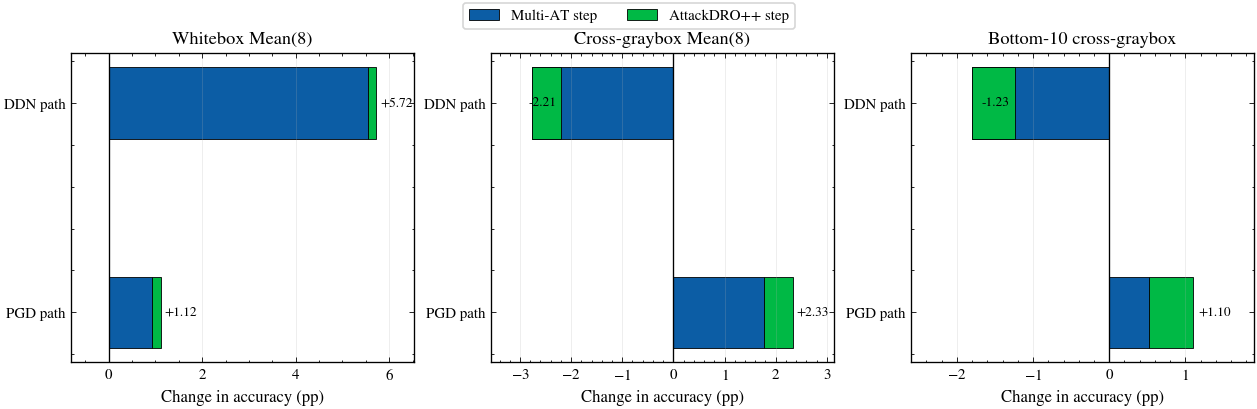
\includegraphics[width=\linewidth]{figures/graybox/method_decomposition_three_panel_science.png}
\caption{Visual decomposition of AttackDRO++ improvement over the
single-attack baselines into a multi-attack effect (Multi-AT
minus single-AT) and a Cluster-DRO effect (AttackDRO++ minus Multi-AT) across whitebox, cross-method graybox, and bottom-10
cross-method graybox metrics, for the two single-AT decomposition
paths.}
\label{fig:ch6_method_decomposition}
\end{figure}

% Section summary removed; transition/closing prose should be written later.
\iffalse
% Disabled graybox section summary removed from the numbered structure.

% TODO[Kiệt]:
% Goal:
% - Remove or convert this section-level summary in a later style cleanup.
% Flow:
% - Replace with a short transition paragraph or move synthesis into `6_summary.tex`.
% Include:
% - No new results.
% Avoid:
% - Keeping section-level summaries against docs/06_style_rules.md.
% Target length: 0 paragraphs here after cleanup; use Chapter 6 summary instead.

The graybox transfer results jointly establish the following
conclusions:

\begin{enumerate}
  \item The graybox random-seed checkpoint panel preserves the whitebox
        trend: it reproduces the Mean(8) ranking AttackDRO++ $>$ Multi-AT
        $>$ PGD-AT $>$ DDN-AT to within $1.0$~pp.
  \item AttackDRO++ improves on Multi-AT by $+0.549$~pp under
        symmetric cross-method graybox transfer at $p \approx 1.1
        \times 10^{-8}$ ($d_z = 0.42$, $n=200$), roughly twice the
        whitebox delta on the same panel. The Cluster-DRO improvement
        therefore strengthens rather than disappears under transfer.
  \item The graybox gain is broad: AttackDRO++ produces a positive
        per-attack delta against Multi-AT on all eight
        evaluation attacks, with five attacks individually significant
        at $p<0.05$ and the largest gain on DeepFool-$\ell_2$
        ($+1.47$~pp, $p<10^{-3}$). It is the only method that meets or
        exceeds Multi-AT on every attack family.
  \item DDN-AT's row-leading graybox accuracy is structural rather
        than substantive.. Its whitebox--graybox gap is $+18.20$~pp,
        roughly twice that of every other method, because $\ell_\infty$
        adversarial examples generated by alternative surrogates
        transfer poorly to a purely-$\ell_2$-trained target. The strong
        graybox row should not be confused with broader robustness;
        DDN-AT's whitebox Mean(8) and Worst(8) remain the lowest of
        the four methods.
  \item The per-cell drilldown shows that AttackDRO++ exceeds        Multi-AT on $59$ of $80$ attack--class cells, with a bottom-10
        lift of $+0.779$~pp on Multi-AT's weakest cells. The
        Cluster-DRO contribution decomposes as approximately $+0.18$~pp
        on whitebox Mean(8), $+0.56$~pp on cross-graybox Mean(8), and
        $+0.80$~pp on the bottom-10 cross-graybox metric, supporting
        the design intent that the objective primarily reshapes
        worst-cell behavior.
\end{enumerate}

These graybox results corroborate the whitebox conclusions of
Section~\ref{sec:ch6_whitebox}: the AttackDRO++ improvement over
Multi-AT reflects a broader cross-attack robustness profile, not a
defense narrowly tuned to its own gradients. The single-attack baselines
remain specialists under both whitebox and graybox attack, and DDN-AT's
apparent graybox strength is exposed as a transfer-mismatch artefact by
the whitebox--graybox gap analysis. The next section examines how these
behaviors emerge during training.
\fi
